% Options for packages loaded elsewhere
\PassOptionsToPackage{unicode}{hyperref}
\PassOptionsToPackage{hyphens}{url}
%
\documentclass[
]{article}
\usepackage{amsmath,amssymb}
\usepackage{iftex}
\ifPDFTeX
  \usepackage[T1]{fontenc}
  \usepackage[utf8]{inputenc}
  \usepackage{textcomp} % provide euro and other symbols
\else % if luatex or xetex
  \usepackage{unicode-math} % this also loads fontspec
  \defaultfontfeatures{Scale=MatchLowercase}
  \defaultfontfeatures[\rmfamily]{Ligatures=TeX,Scale=1}
\fi
\usepackage{lmodern}
\ifPDFTeX\else
  % xetex/luatex font selection
\fi
% Use upquote if available, for straight quotes in verbatim environments
\IfFileExists{upquote.sty}{\usepackage{upquote}}{}
\IfFileExists{microtype.sty}{% use microtype if available
  \usepackage[]{microtype}
  \UseMicrotypeSet[protrusion]{basicmath} % disable protrusion for tt fonts
}{}
\makeatletter
\@ifundefined{KOMAClassName}{% if non-KOMA class
  \IfFileExists{parskip.sty}{%
    \usepackage{parskip}
  }{% else
    \setlength{\parindent}{0pt}
    \setlength{\parskip}{6pt plus 2pt minus 1pt}}
}{% if KOMA class
  \KOMAoptions{parskip=half}}
\makeatother
\usepackage{xcolor}
\usepackage[margin=1in]{geometry}
\usepackage{color}
\usepackage{fancyvrb}
\newcommand{\VerbBar}{|}
\newcommand{\VERB}{\Verb[commandchars=\\\{\}]}
\DefineVerbatimEnvironment{Highlighting}{Verbatim}{commandchars=\\\{\}}
% Add ',fontsize=\small' for more characters per line
\usepackage{framed}
\definecolor{shadecolor}{RGB}{248,248,248}
\newenvironment{Shaded}{\begin{snugshade}}{\end{snugshade}}
\newcommand{\AlertTok}[1]{\textcolor[rgb]{0.94,0.16,0.16}{#1}}
\newcommand{\AnnotationTok}[1]{\textcolor[rgb]{0.56,0.35,0.01}{\textbf{\textit{#1}}}}
\newcommand{\AttributeTok}[1]{\textcolor[rgb]{0.13,0.29,0.53}{#1}}
\newcommand{\BaseNTok}[1]{\textcolor[rgb]{0.00,0.00,0.81}{#1}}
\newcommand{\BuiltInTok}[1]{#1}
\newcommand{\CharTok}[1]{\textcolor[rgb]{0.31,0.60,0.02}{#1}}
\newcommand{\CommentTok}[1]{\textcolor[rgb]{0.56,0.35,0.01}{\textit{#1}}}
\newcommand{\CommentVarTok}[1]{\textcolor[rgb]{0.56,0.35,0.01}{\textbf{\textit{#1}}}}
\newcommand{\ConstantTok}[1]{\textcolor[rgb]{0.56,0.35,0.01}{#1}}
\newcommand{\ControlFlowTok}[1]{\textcolor[rgb]{0.13,0.29,0.53}{\textbf{#1}}}
\newcommand{\DataTypeTok}[1]{\textcolor[rgb]{0.13,0.29,0.53}{#1}}
\newcommand{\DecValTok}[1]{\textcolor[rgb]{0.00,0.00,0.81}{#1}}
\newcommand{\DocumentationTok}[1]{\textcolor[rgb]{0.56,0.35,0.01}{\textbf{\textit{#1}}}}
\newcommand{\ErrorTok}[1]{\textcolor[rgb]{0.64,0.00,0.00}{\textbf{#1}}}
\newcommand{\ExtensionTok}[1]{#1}
\newcommand{\FloatTok}[1]{\textcolor[rgb]{0.00,0.00,0.81}{#1}}
\newcommand{\FunctionTok}[1]{\textcolor[rgb]{0.13,0.29,0.53}{\textbf{#1}}}
\newcommand{\ImportTok}[1]{#1}
\newcommand{\InformationTok}[1]{\textcolor[rgb]{0.56,0.35,0.01}{\textbf{\textit{#1}}}}
\newcommand{\KeywordTok}[1]{\textcolor[rgb]{0.13,0.29,0.53}{\textbf{#1}}}
\newcommand{\NormalTok}[1]{#1}
\newcommand{\OperatorTok}[1]{\textcolor[rgb]{0.81,0.36,0.00}{\textbf{#1}}}
\newcommand{\OtherTok}[1]{\textcolor[rgb]{0.56,0.35,0.01}{#1}}
\newcommand{\PreprocessorTok}[1]{\textcolor[rgb]{0.56,0.35,0.01}{\textit{#1}}}
\newcommand{\RegionMarkerTok}[1]{#1}
\newcommand{\SpecialCharTok}[1]{\textcolor[rgb]{0.81,0.36,0.00}{\textbf{#1}}}
\newcommand{\SpecialStringTok}[1]{\textcolor[rgb]{0.31,0.60,0.02}{#1}}
\newcommand{\StringTok}[1]{\textcolor[rgb]{0.31,0.60,0.02}{#1}}
\newcommand{\VariableTok}[1]{\textcolor[rgb]{0.00,0.00,0.00}{#1}}
\newcommand{\VerbatimStringTok}[1]{\textcolor[rgb]{0.31,0.60,0.02}{#1}}
\newcommand{\WarningTok}[1]{\textcolor[rgb]{0.56,0.35,0.01}{\textbf{\textit{#1}}}}
\usepackage{graphicx}
\makeatletter
\def\maxwidth{\ifdim\Gin@nat@width>\linewidth\linewidth\else\Gin@nat@width\fi}
\def\maxheight{\ifdim\Gin@nat@height>\textheight\textheight\else\Gin@nat@height\fi}
\makeatother
% Scale images if necessary, so that they will not overflow the page
% margins by default, and it is still possible to overwrite the defaults
% using explicit options in \includegraphics[width, height, ...]{}
\setkeys{Gin}{width=\maxwidth,height=\maxheight,keepaspectratio}
% Set default figure placement to htbp
\makeatletter
\def\fps@figure{htbp}
\makeatother
\setlength{\emergencystretch}{3em} % prevent overfull lines
\providecommand{\tightlist}{%
  \setlength{\itemsep}{0pt}\setlength{\parskip}{0pt}}
\setcounter{secnumdepth}{-\maxdimen} % remove section numbering
\ifLuaTeX
  \usepackage{selnolig}  % disable illegal ligatures
\fi
\IfFileExists{bookmark.sty}{\usepackage{bookmark}}{\usepackage{hyperref}}
\IfFileExists{xurl.sty}{\usepackage{xurl}}{} % add URL line breaks if available
\urlstyle{same}
\hypersetup{
  pdftitle={Week 2 - OpenRefine},
  pdfauthor={Emil Bæk Mogensen},
  hidelinks,
  pdfcreator={LaTeX via pandoc}}

\title{Week 2 - OpenRefine}
\author{Emil Bæk Mogensen}
\date{2023-09-14}

\begin{document}
\maketitle

\textbf{Packages}

```\{r\} library(tidyverse) library(tinytex) library(knitr) ````

\begin{enumerate}
\def\labelenumi{\arabic{enumi})}
\tightlist
\item
  \textbf{Create a \emph{tidy} spreadsheet/table listing the names of
  Danish monarchs with their birth- and death-date and duration of
  reign. They should be sortable by year of birth. Suitable source
  websites are here and here, but you can also use another source,
  provided you reference it.}
\end{enumerate}

The source I decided to use was the one from the
\href{https://www.kongehuset.dk/monarkiet-i-danmark/kongerakken}{official
website of the Royal Danish House}, which has a far deeper description
of the monarchs compared to the English url. As it was not possible to
upload the data directly into OpenRefine with the URL option, I decided
to webscrape
\href{https://github.com/Emil3103/Digital-Methods/blob/main/Week_02/Data/danish_monarchs_data.csv}{the
data}. Afterwards I cleaned/tidy'ed it to a point where i could finish
it manually in excel:. The script to track these steps up until the
manual finishing can be found in my
\href{https://github.com/Emil3103/Digital-Methods/blob/main/Week_02/Scripts/danish_monarchs_openrefine}{GitHub}
Lastly, i decided to remove interregnums and periods where the throne
was contested by multiple kings in the
\href{https://github.com/Emil3103/Digital-Methods/blob/main/Week_02/danish_monarchs_sheet.xlsx}{spreadsheet}.

\begin{enumerate}
\def\labelenumi{\arabic{enumi})}
\setcounter{enumi}{1}
\tightlist
\item
  \textbf{Does OpenRefine alter the raw data during sorting and
  filtering?}
\end{enumerate}

Sorting and filtering does not alter the data. OpenRefine maintains the
integrity of the raw data as it simply allows transformations and
editing, which in itself allows experimentation without fear of getting
lost in the approach or ruining the data.

\begin{enumerate}
\def\labelenumi{\arabic{enumi})}
\setcounter{enumi}{2}
\tightlist
\item
  \textbf{Fix the interviews dataset in Openrefine enough to answer this
  question: Which two months are reported as the most
  water-deprived/driest by the interviewed farmer house-holds?}
\end{enumerate}

After following and doing the carpentry lesson for the social sciences'
i found that the most water-deprived months reported by the farmer
households were October and September with 74 and 70 reports
respectively. Firstly, I created a custom text facet using the
value.replace function to clean the dataset of ``{[}{[},.'' leaving only
the abbreviation ``xxx'' separated by a semicolon of the months in the
column. Secondly, I used the ``split multi-varied cells'' with semicolon
separator. Lastly, I clustered the words and got the following
picture.\\
The step-by-step approach can be found at my
\href{https://github.com/Emil3103/Digital-Methods/blob/main/Week_02/Scripts/danish_monarchs_openrefine}{GitHub.}

\href{https://github.com/Emil3103/Digital-Methods/blob/main/Week_02/Screenshots/months_no_water.png}{\includegraphics{images/months_no_water-01.png}}

\begin{enumerate}
\def\labelenumi{\arabic{enumi})}
\setcounter{enumi}{3}
\tightlist
\item
  \textbf{OPTIONAL Real-Data-Challenge: What are the 10 most frequent
  occupations (erhverv) among unmarried men and women in 1801 Aarhus?
  (hint: some expert judgement interpretation is necessary)}
\end{enumerate}

I began by using the URL upload option in Openrefine. Firstly, I applied
a text filter with the word ``ugift'' on the ``civilstand'' column.
Secondly, I decided to split the column with the regex:

\begin{Shaded}
\begin{Highlighting}[]
\CommentTok{\# ,|\textbackslash{}bog}
\end{Highlighting}
\end{Shaded}

This gave me three columns total, of which i focused on the ``erhverv
1'' column because it is indicated, and thus highly assumed, that this
is peoples primary occupancy. Thirdly, I created text facet for the
``Erhverv column.'' I decided to cluster by occupancy in the broadest
sense e.g.~that of ``soldier'' for anyone within the military, thus
leaving out company, rank and specialty within occupancy. After not
being able to do any more of the clustering options, i got the following
result.

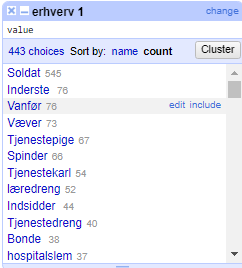
\includegraphics{images/erhverv_1_.png}

Although I was asked to focus on the ``erhverv'' column, I realized by
going through it that there were huge discrepancies in the way people
responded. This lead me to looking through neighbouring columns, as I
was reminded by the carpentry lessons that these mistakes were possible.
I found that by clustering the ``famstand'' column, although most rows
were related to the actual column headline, it had many rows filled with
occupancy. Although i swam into deep water and ran into multiple errors
and unresponsiveness from OpenRefine in my quest to uncover it, there is
no doubt that the occupancy of servant for both men and females
respectively was the most frequent. The step-by-step approach to the
imported data set can be found at my
\href{https://github.com/Emil3103/Digital-Methods/blob/main/Week_02/Scripts/occupany_openrefine.json}{GitHub.}

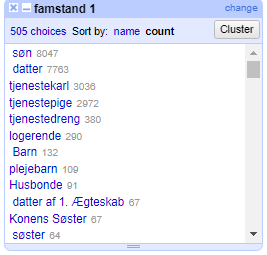
\includegraphics{images/famstand_1.PNG}

\end{document}
